%%%%%%%%%%%%%%%%%%%%%%%%%%%%%%%%%%%%%%%%%%%%%%%%%%%%%%
\section{はじめに}

 電離圏研究のために実施されている短波ドップラー(HFD)観測のデータはオープンデータとして公開されており,自由な使用が認められている.
現状,データ活用を促進するために数件の web アプリケーションが開発されているが,多くが開発運用の困難性やユーザーエクスペリエンス等の観点で問題を抱えている.
 この課題点を解消するため既存のアプリケーションの課題点から必要要件を洗い出し,ページレンダリング手法を考慮した web アプリケーションの新規設計を行う.本研究ではその中の web スクレイピングを用いてデータを取得する処理,および,取得したデータを整形して扱いやすくする処理に焦点を当て研究を行う.
本研究ではNext.jsと呼ばれるフレームワークを用いて実装を行う.JavaScriptのUIライブラリの一つであるReact.jsがベースとなっており,サーバ機能も有しているため効率的なweb開発が可能である.また,使用する言語を統一して管理コストの低減を図るため,webスクレイピングはTypeScriptを用いて行う.
%%%%%%%%%%%%%%%%%%%%%%%%%%%%%%%%%%%%%%%%%%%%%%%%%%%%%%
\section{Webスクレイピングについて}

 webスクレイピングとは,web サイトから情報を抽出するコンピュータソフトウェア技術のことを指す.HTML フォーマットからテキストを抽出してスプレッドシートや json ファイル等の構造化データへの変換を行うことができ,web 上にあるデータを取得して扱うことを目的とする.web スクレイピングの手法としては,正規表現や DOM 解析,HTML パーサ等を用いたものがある.本研究では,ISRを用いたwebアプリケーションを設計するため,スクレイピングの処理に速度を求める必要がない.そのため,本研究では軽量でサーバへの負担が小さいcheerioをHTMLパーサとして用いる.
%%%%%%%%%%%%%%%%%%%%%%%%%%%%%%%%%%%%%%%%%%%%%%%%%%%%%%
\section{使用ライブラリ}
 本研究で使用した主なTypeScritpライブラリについて以下に示す.
%%%%%%%%%%%%%%%%%%%%%%%%%%%%%%%%%%%%%%%%%%%%%%%%%%%%%%
\subsection{Superagent}

 HTMLリクエストを送信することのできるモジュール.本研究ではHFD観測データが公開されているwebページからHTMLレスポンスとしてテキストデータを取得する際に用いる.\cite{superagent}
%%%%%%%%%%%%%%%%%%%%%%%%%%%%%%%%%%%%%%%%%%%%%%%%%%%%%%
\subsection{Cheerio}

 HTMLパーサにjQueryのサブセットを実装したもの.jQueryの関数を用いてスクレイピングの処理を行うことができる.本研究ではHTMLレスポンスからテキストデータだけを抜き出す際に用いる.\cite{cheerio}
%%%%%%%%%%%%%%%%%%%%%%%%%%%%%%%%%%%%%%%%%%%%%%%%%%%%%%
\section{実装}
%%%%%%%%%%%%%%%%%%%%%%%%%%%%%%%%%%%%%%%%%%%%%%%%%%%%%%
\subsection{目標}
 本開発では,Next.jsを用いて開発運用及びユーザーエクスペリエンスの観点で従来のものよりも優れたWebアプリケーションを作成することを目標とする.その中でも,本研究ではスクレイピングを用いてデータを取得し,それをフロントエンドで扱いやすいように整形する処理を行うことまでを目標とする.
%%%%%%%%%%%%%%%%%%%%%%%%%%%%%%%%%%%%%%%%%%%%%%%%%%%%%%
\subsection{スクレイピング処理}
 Superagentを用いて,HFドップラーのデータが公開されているwebサイト\cite{hfd}にHTMLリクエストを送る.返ってきたHTMLレスポンスからcheerioを用いてbodyを抜き出し,テキストデータに変換する.
%%%%%%%%%%%%%%%%%%%%%%%%%%%%%%%%%%%%%%%%%%%%%%%%%%%%%%
\subsection{データ整形処理}
 前項で取得したテキストデータはそのままでは扱いにくいため,扱いやすい形に整形する.例として,2020/11/20Sarobetsuというデータを示す.
 \begin{figure}[h]
   \centering
   \caption{Caption}
   \label{fig:my_label}
   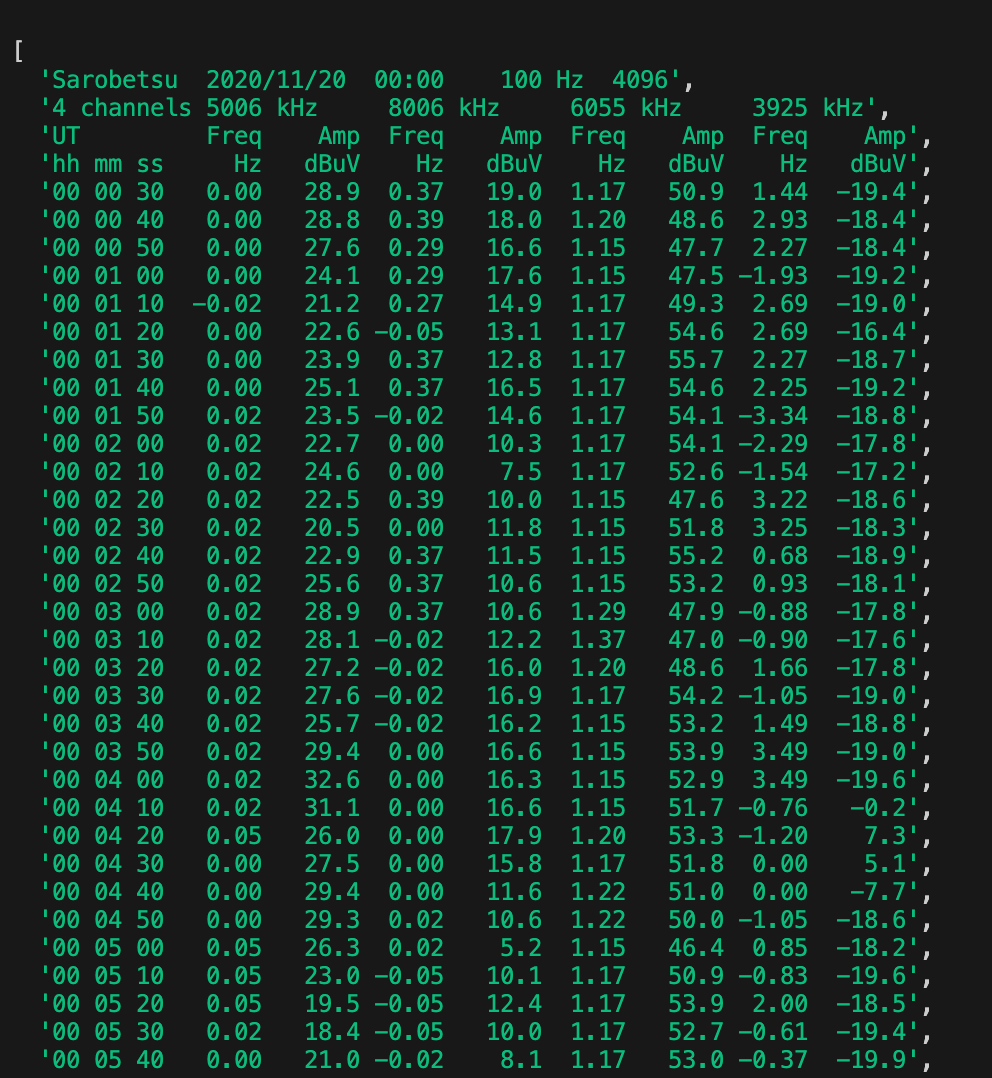
\includegraphics[width=70mm]{fig/textdata.png}
 \end{figure}
%%%%%%%%%%%%%%%%%%%%%%%%%%%%%%%%%%%%%%%%%%%%%%%%%%%%%%
\subsection{完成品}
 完成したサイトがこちらになります.
%%%%%%%%%%%%%%%%%%%%%%%%%%%%%%%%%%%%%%%%%%%%%%%%%%%%%%
\small
\begin{thebibliography}{99}
\setlength{\itemsep}{0pt}
\smallskip

\bibitem{shu_sotsuken}
中嶋柊,HF ドップラー観測データの利活用を目的とする web アプリケーションのフロントエンド設計,令和4年度 制御情報システム創造演習 報告書

\bibitem{superagent}
Superagent-npm 
\url{https://www.npmjs.com/package/superagent}  2023/01/25

\bibitem{cheerio}
cheeriojs/cheerio: Fast, flexible, and lean implementation of core jQuery designed specifically for the server. 
\url{https://github.com/cheeriojs/cheerio}  2023/01/25 

\bibitem{hfd}
HF Doppler Sounding Experiment in Japan - HFDOPE
\url{http://gwave.cei.uec.ac.jp/~hfd/pre.html} 2024/

\end{thebibliography}
\normalsize
%%%%%%%%%%%%%%%%%%%%%%%%%%%%%%%%%%%%%%%%%%%%%%%%%%%%%%





